\documentclass[12pt]{article}
% \usepackage[margin=1in]{geometry}
\usepackage{graphicx, url}

\title{Raising An Axe to the Axioms \\ \small An investigation into the definition and foundations of mathematics before the European renaissance}
\author{Joel Savitz}

\begin{document}
\maketitle

% 1. What is mathematics? What does that question mean?

\section{Introduction}

Mathematics ---
an art invisibly fundemental to society
and yet misunderstood most by its most adept practitioners.
As one of the building blocks of civilization,
the history of mathematics provides an upper bound
to the complexity of any society.
Long practiced formally by the educated elite
and informally by the laborer,
the students of the modern classroom
are taught mathematics from the earliest age
that adults consider them able.
One may conclude by their common sense
that the definition of this universal art
would be a matter of consensus,
as for most that conclusion corresponds
with the manner in which they have been taught,
a set of computational techniques to memorize and
perhaps a set of tools to use to solve problems.
One with faith in such a conclusion
may be surpised to learn that
no such consensus exists \cite{tobies}.

The controversy extends
beyond simply the definition.
Mathematicians disagree on even
basic questions
about the nature of the subject
and its fundamental essence,
such as whether mathematical ideas
are constructed or discovered,
what activity constitutes mathematics,
and the relation of the subject
to other areas of study.
In this paper,
I will give a brief overview
of the history of the definition of mathematics
and its purpose in various ancient societies,
as well as a look at a few often overlooked
medieval developments that predate the renaissance.

For brevity, the scope of this paper
will be limited mostly
to Western history,
but a comprehensive treatment of this subject
would not rely on such a narrow constraint.

\section{Origins}

The birth of mathematical practice
--- like many of the primitive civilizational arts ---
is cloaked in the mist of prehistory.
The oldest known records indicate its
invention by reason of necessity.
As the human being arose from the animal kingdom
and began to plan for the future,
hunter-gatherer societies developed
a need to measure the passage of time.
The earliest record of such an attempt
was discovered in Africa in 1960.
Known as the Ishango bone,
this 20,000-25,000 year-old artifact
displays a pattern of groves and notches.
While some consider the mammalian bone
to be a simply tally stick \cite{ishango},
others suggest that it might be a diagram
depicting the phases of the moon \cite{ishango2}.
I invite the reader to take a look at figure \ref{fig1}
and make their own judgement.

\begin{figure}
	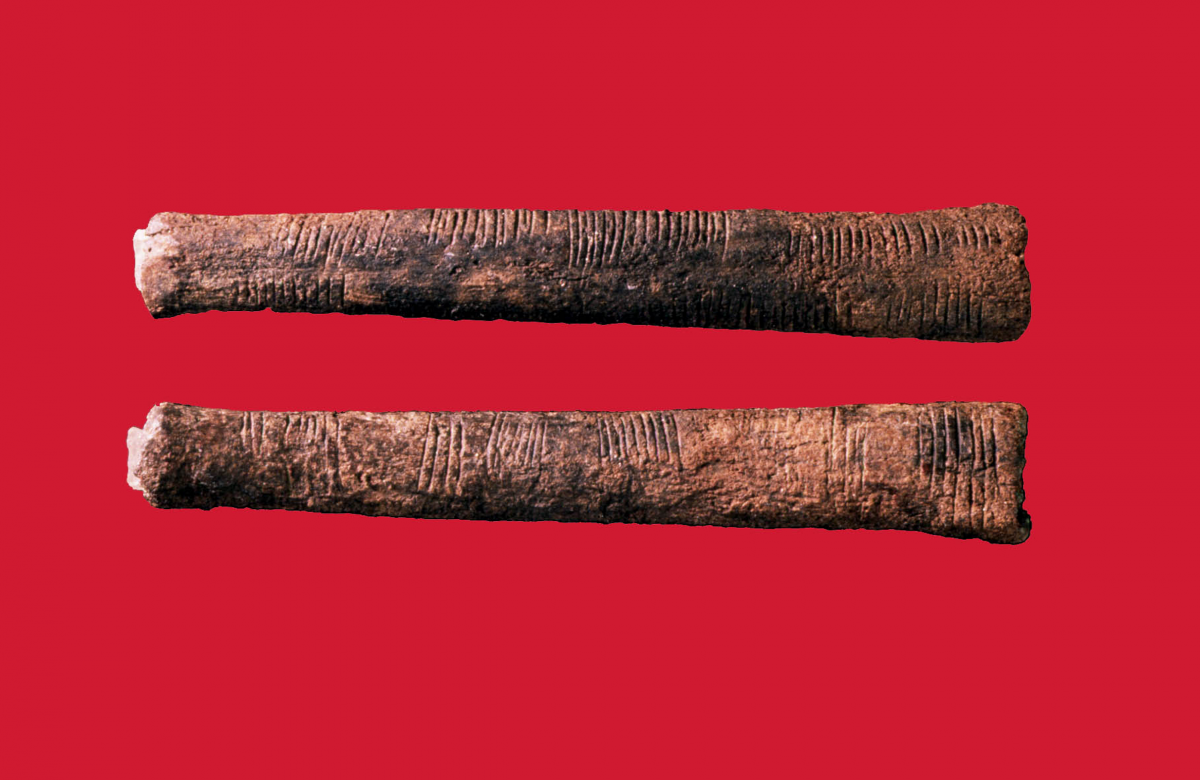
\includegraphics[scale=0.28]{ishango.png}
	\centering
	\caption{The Ishango Bone \cite{ishango}}
	\label{fig1}
\end{figure}

We can only speculate
as to the extent of mathematical thought
that is lost to history,
either in the form of a lost oral tradition
or destroyed document.
Some professional and amateur historians
may speculate otherwise,
but the earliest undisputed documents
date back to ancient Sumerian metrology.
This usage appears to be fundamentally practical,
and this is demonstrated by their used of
a sexagesimal number system,
later adopted by their Babylonian successors \cite{boyer1991}.
Similar motivations appear to have inspired the Egyptians,
as the bureaucracy needed a technique
to manage a complex agricultural system.
Far fewer mathematical documents survive
from earlier Egyptian society,
but the Rhind Mathematical Papyrus,
dating back to approximately 1550 BCE,
demonstrates --- from the perspective of
the ancient scribe Ahmose ---
how to solve eighty-four problems
via a practical technique \cite{rhind}.
This is further evidence for the mostly
practical and necessity-based nature
of early mathematics.

% TODO: fix chinese section or cut?
% Perhaps the ancient Chinese practitioners
% of this art would beg to differ,
% but unfortuantely due to a 212 BCE order
% of Emperor Qin Shi Huang,
% all non-sanctioned books were to be burned.
% This was of course far from universily obeyed,
% but our modern knowledge of ancient Chinese mathematics
% has been limited due to this
% unfortuante abuse of power


% 2. What did the ancients think of the nature of math?

% 2a. Egyptians, Greeks, Chinese, etc

\section{Theoretical development}

In ancient Greece,
we see the emergence of mathematics
as a fundamental partner of philosophy.
``Tradition'' ascribes the following phrase
to an engraving above Plato's Academy,
``Let no one ignorant of geometry enter''.
Despite the unfortunate reality that
our earliest reliable sources for this inscription
appear roughly ten centuries after Plato's death \cite{plato_truth}
and long after Justinian's order to close
the Academy in 529 CE, 
the spirit of the statement is evident
in the work of Plato himself,
for he states in the Republic that
``studies that demand more toil
in the learning and practice than this
we shall not discover easily
nor find many of them'',
with reference to
the study of geometry \cite{plato}.
Indeed, it is Plato that established ---
in the West ---
the tradition of placing great importance
on mathematical education
for its own sake.
He considered it essential
for the development
of the mind of the human
and its capacity for abstraction.
Plato made no significant mathematical discoveries,
with the notable exception of the identification
of the platonic solids.
Rather, his importance to
the history of the definition of mathematics
is due to the ideological revolution he propagated,
for it is his insistence on the relationship between
mathematics and philosophy
and his emphasis on the importance of free inquiry
that forms the very axe which we raise
to the axioms of his successors.

The history of
Greek deductive reasoning
predates and outlives Plato.
Aristotle attributes
the origin of
Greek philosophy
to Thales of Miletus \cite{aristotle_thales},
and he is the first known
individual to use
deductive reasoning in a geometric context,
as well as the first to be credited
with a mathematical discovery \cite{boyer1991}.
Thales, by his example,
paved the way for centuries of Greek pre-science,
pulling back the curtain of mythological fantasy
with both hands,
one fist of natural philosophy,
and another of deductive geometry.
Centuries of discovery proceeded,
from the triangles of Archimedes
to the number theory of Diophantus,
but the undoubtable crescendo
was the Alexandrian Euclid.
His \textit{Elements} summarized
centuries of Greek progress in Mathematics
and served as the most popular
and influential mathematics textbook of all time,
only being superseded around the late 19th century \cite{boyer1991}.

We see in \textit{Elements} a great achievement
in the history of rigorous reasoning.
The textbook formalizes the axiomatic method,
a landmark achievement of the human being that
--- I would argue ---
deserves similar respect to the scientific method,
for the former does for \textit{a priori} objectivity
what the latter does for \textit{a posteriori} objectivity.
The seed of a giant of rigor is planted by Euclid,
and mathematicians ever since have stood on its shoulders.
Euclid introduced countless students to methods such as
direct proof, reductio ad absurdum, and basic number theory.
One can only speculate as to the benefit enjoyed by
the human being as a result of this text.
Beyond mathematical technique,
and very much following in the Platonic tradition
of the study thereof as an end in itself,
human minds sharpened by the study of Euclid
have pierced the veil of numerous fields
beyond mathematics.
Einstein called the Elements
his ``holy little geometry book'' \cite{einstein},
and by the sheer number of
translations, publications, and enthusiasts,
as well as a zealous set of followers,
this allusion
--- which in my opinion compares the importance of the \textit{Elements}
to that of the Bible ---
is far from unfounded.

Reverence for mathematics had in fact
become a religion of its own
for one particular bean-eschewing
cult founded by a man with a theorem
so eponymous that for many non-mathematicians,
the Pythagorean theorem is as well known to them
as the fact that the mitochondria is the powerhouse of the cell.
As an example of the pop cultural significance of the Pythagoreans,
I invite the reader in need of a laugh to feast their eyes upon figure \ref{fig2}.


\begin{figure}
	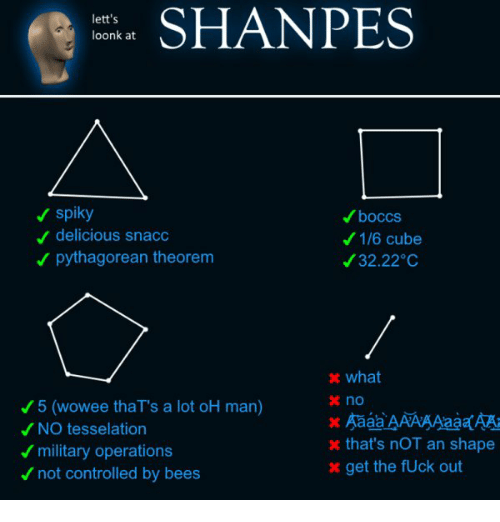
\includegraphics[scale=0.4]{shanpes.png}
	\centering
	\caption{Let's look at Shapnes (Meme/Art) \cite{shanpes}}
	\label{fig2}
\end{figure}


Pythagoras ---
incidentally a contemporary of Confucious ---
was both a mathematician and prophet.
Few documents survive from his time period,
but historians have reached a consensus on certain points
of his life and the activity
of his eponymous secret society.
His cult is described as similar in form to Orphism
but based in mathematics and philosophy.
Pythagoras is even credited with
the coinage of these very terms,
though many of the important discoveries
bearing his name,
are believed to be discovered by
unknown cult-members and held in common \cite{boyer1991}.
This rare entanglement of religion and mathematics
provides an alternative perspective on
the ancient definition of the art.
In contrast to the Ionian school of Thales,
mathematics was not a technique
to dispel mythological superstition,
rather it was a mystical technique in itself.
Take for instance the Pythagorean Tetractys,
depicted in figure \ref{fig3}.
Dantzig relates the following prayer,
addressed by the Pythagorean worshipers
to the shape of the Tetractys itself
with great reverence:


\begin{figure}
	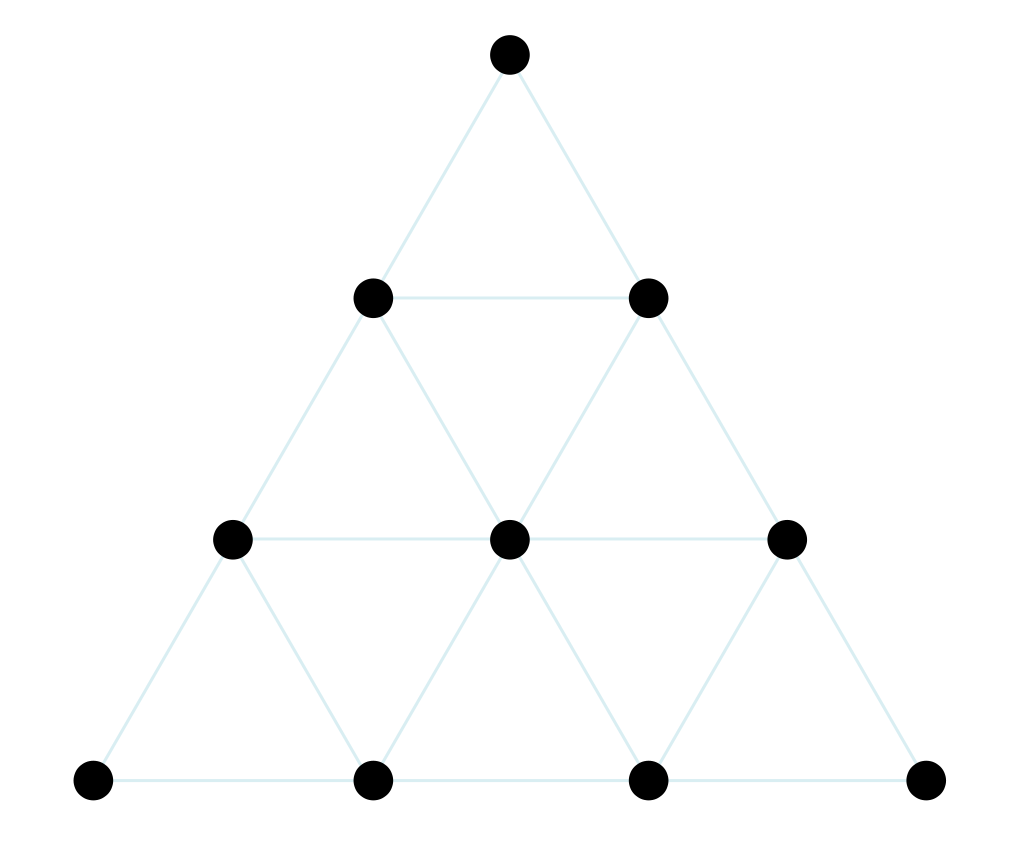
\includegraphics[scale=0.1]{tetractys.png}
	\centering
	\caption{The (holy?) Tetractys \cite{tetractys}}
	\label{fig3}
\end{figure}

\begin{quote}

	Bless us, divine number, thou who generated gods and men! O holy, holy Tetractys, thou that containest the root and source of the eternally flowing creation! For the divine number begins with the profound, pure unity until it comes to the holy four; then it begets the mother of all, the all-comprising, all-bounding, the first-born, the never-swerving, the never-tiring holy ten, the keyholder of all \cite{dantzig}.

\end{quote}

One voice inside of me finds it difficult to relate
to this ancient superstition,
but this voice gets strangely quiet
when I am engrossed in a difficult problem.
In those moments of creative flow
and arguably elevated consciousness,
I can see the Pythagorean perspective.
Perhaps not in fourfoldness,
but certainly in the sublime nature of mathematical beauty.

Plato and Aristotle,
influenced by Pythagorean mysticism,
integrated these ideas
into their insistence that mathematical understanding 
is the fundamental building block of higher questions.
Indeed, their conception of the universe as
being in a harmonic order is arguably derived from
Pythagorean beliefs about music
and the seemingly perfect ratio between certain notes.

We can describe the ancient definitional controversy
with these two broad strokes.
On one hand, mathematics is the basis of free scientific inquiry,
dispelling superstition and mythology
and providing a rational basis for prescience.
On the other hand, mathematics is itself a spiritual tool,
providing insight into mystical metaphysical realms
and a glimpse beyond the physical world.
Viewed from a certain anggle,
this dichotomy has a correspondence with one of
the fundamental definitional dichotomies
of modern math,
the question of whether mathematical concepts
are discovered or invented.
If math is invented,
then it is one of the greatest constructions of the human being,
providing a basis for nearly all other constructions and creations,
demonstrating the power of human creativity
and the ability of the human to rise beyond the animal constraints of the mind
so imposed and hardwired by the primordial evolutionary conditions.
If math is discovered,
then it is one of the greatest mysteries the human has uncovered,
a secret truth so fundamental to the universe
that the study of the art corresponds
with later \textit{a posteriori} scientific discovery
long before the necessary observations and deductions are made.

Mathematics virtually disappears from Western Europe,
along with literacy and scholarship,
following the decline and fall of the Roman empire.
Though the art thrived in many more sophisticated
parts of the world throughout the period
following the collapse,
I would argue that mathematics reappears in Western Europe
far earlier than most give credit.
The traditional history of Western European civilization,
twisted by the early Italian renaisaince rejection
of catholic dogma in all its forms,
may have thrown out important chunks of baby
with its dank, superstitious bathwater.

Euclid reappears in Western Europe
in the twelfth century
thanks to Adelard of Bath,
who visited Islamic Spain
and made the translation
from Arabic to Latin,
introducing the lost axiomatic method of the ancients
to the monastic orders of Europe,
who --- though highly superstitious
and constrained by the Catholic Church ---
began to revive the Academic tradition
of Plato and Aristotle during the Scholastic movement
of that and the following century \cite{russell}.
Russell --- a great mathematician himself ---
criticizes the Scholastics for their obsession
with dialectic, even in contradiction to observational evidence.
Certainly this is unscientific and this manner of thinking
is a dead end for much of natural philosophy,
but their emphasis on ``verbal distinctions and subtleties''
and intense focus on derivations from an infallible
scripture appear as a pre-mathematics in parallel
to the reappearance of Euclid in the west.
Ab\'elard, a medieval French Scholastic,
serves as a prime example of this pre-renaissance renaissance
in axiomatic rigor.
Despite a striking and unfortunate disdain for empiricism,
his book ``Yes and No'',
composed in the early twelfth century,
attempts to argue for numerous theses,
not so much in order to reach a conclusion
as to demonstrate
the beauty and importance 
of argument itself.
He was such a fanatic of Logic
that he considered it to be the
most Christian of the sciences,
and compared the word to the Christian
conception of Jesus as the Greek Logos,
the terminology used in Saint John's gospel \cite{russell}.

This is a definitional novelty in the history of mathematics.
Despite the vast intellectual oppression of Catholic dogma,
the imposed constraints of scripture served as state-mandated axioms,
and rigorous, narrow, systematic \textit{a priori} reasoning
was applied to this non-numerical and non-geometric
system of thought,
introducing a new vector of abstraction
in the very axioms of the system itself.
To Euclid, an axiom was simply a common notion
that anyone could ---
and should ---
accept as true before actual argument,
and to the Scholastics, scripture and dogma served
as axioms themselves, as they had little ideological choice.
Even in contrast to the Pythagoreans this was novel,
as it was not number and form that served as the metaphysical basis,
rather it was dialectical study of a non-numerical axiomatic system,
applying the methods of mathematics to a previously non-mathematical context.
This ideological novelty appears far before the more famous usage
of non-numerical analysis of our time,
that of the analysis of algorithm,
and perhaps this early medieval study of precision in verbal subtlety
and systematization of non-numerical argument
contributed to later systems of thought as vast as formal language theory
and alternative axiomatic systems.
If so, this is a relatively unknown revolution in mathematical thinking,
as the death of certainty in scripture in later European academia
drained these arguments of their ideological weight
while preserving their rigor as isolated abstractions,
consistent only within the context of their own argumentative reasoning
but disconnected to the greater universe.
This is the modern notion of an axiomatic system,
and perhaps the medieval Scholastics deserve more credit than they are given.

\section{Conclusion}

Unfortunaltely, we set down our axe
before the forest has fully grown.
Mathematical complexity exploded
parallel to the scientific revolution,
and development of the axiomatic method
and rigorous foundations for mathematics
co-developed with scientific rigor.
The two great areas of endeavor
appear to be fundamentally entwined,
as Wigner argues in his 1960 article
on the ``Unreasonable Effectiveness
of Mathematics in the Natural Sciences''.
Mathematicians often find pure mathematical results
that are only later found to be applicable
to some aspect of the natural world \cite{wigner}.

At the same time,
mathematics has its controversies.
Most of what we call modern mathematics
is founded ---
sometimes explicitly but often implicitly ---
in the Zermelo-Fraenkel set theory axioms,
generally including an additional axiom
known as the axiom of choice.
As demonstrated by the Scholastics,
the axiomatic method can be applied to
areas of study beyond the numeric and geometric,
and as proponents of alternative foundations
such as Homotopy Type Theory argue,
modern mathematics can and perhaps should
move past the default choice of a set-theoretic foundation \cite{ladyman}.
Unlike the scripture of
those tireless medieval monk,
modern mathematics was not delivered
in complete and perfect form
to a prophet on a mountain
to be forever engraved in stone.
Rather, the story of mathematics
continues to be written and debated,
with control of the art resting
in the hands of
no single individual.
Mathematics is the collective complexity
of the human being
and like the human,
its greatest quality
is its capacity to change.


% \section{Rigorous foundations}

% 3. The renaissance of math (classical to 18th century]

% 4. Motivation for formal foundations (19th century)

% 4a. Peano axioms, Russell's paradox, Cantor and uncountability

% 5. 20th century definitions

% 5a. Axiomatic Set theory and modern mathematical foundations

% 5b. Logicism, Intuitionism, Formalism, and a few other schools of thought

% 6. Alternative foundations of mathematics

% 6a. Criticism of ZFC and ultrafinitism (NJ wildberger)

% 6b. Intensional type theory vs extensional set theory (Russell, Martin-Löf)

% 6c. The computer science revolution

% \section{Defining the future}

% We live in an ever more golden age of mathematics.

% \begin{itemize}
% 	\item teaching to all students
% 	\item pedagogical research
% 	\item exploding dots for example
% 	\item youtubers like 3b1b, flaming maths, mathologer
% 	\item computers...
% \end{itemize}

% 7. How should we define mathematics?

% 7a. My personal definition

% 7b. Connections to mathematics education

% 7c. Remaining questions

\bibliographystyle{plain}
\bibliography{paper}

\end{document}
